\documentclass[margin,line]{res}
\usepackage{hyperref}
\usepackage{url}
\usepackage{graphicx}
\usepackage{xcolor}
\usepackage{ragged2e}
\oddsidemargin -.5in
\evensidemargin -.5in
\textwidth=6.0in
\itemsep=0in
\parsep=0in
\topmargin=0in
\topskip=0in
 
\newenvironment{list1}{
  \begin{list}{\ding{113}}{%
      \setlength{\itemsep}{0in}
      \setlength{\parsep}{0in} \setlength{\parskip}{0in}
      \setlength{\topsep}{0in} \setlength{\partopsep}{0in}
      \setlength{\leftmargin}{0.17in}}}{\end{list}}
\newenvironment{list2}{
  \begin{list}{$\bullet$}{%
      \setlength{\itemsep}{0in}
      \setlength{\parsep}{0in} \setlength{\parskip}{0in}
      \setlength{\topsep}{0in} \setlength{\partopsep}{0in}
      \setlength{\leftmargin}{0.2in}}}{\end{list}}



    
\begin{document}
\pagecolor{blue!10}
\begin{figure}
\hspace{1.7in}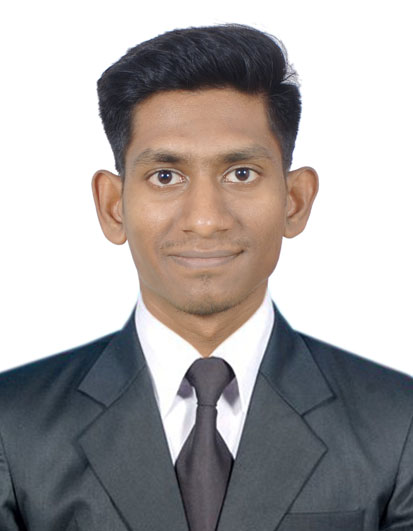
\includegraphics[width=0.25\textwidth]{DSC_8914}
\end{figure}

\name{\LARGE Kezhakkepurakkel Niraj K. Venugopal} \hfill {\em \today}

\begin{resume}
\section{\sc Contact Information}

\vspace{.05in}
\begin{tabular}{@{}p{3.5in}p{3in}}
Student            & {Phone:}  (+91) 7698075665 \\
A-4, Satyam Tenament 
 & {E-mail:}  nirajkvenugopal@gmail.com\\
Bajwa - Karodiya Road, \\
Karodiya, Gujarat.  
\end{tabular}

\hspace{.5in}{LinkedIn ID:} \url{linkedin.com/in/niraj-k-venugopal-88a128169/}


\section{\sc Interests}

 Designing and Analysis, 3D Printing, Research and  Development

\section{\sc Education}
{\bf Vadodara Institute Of Engineering}, Vadodara, Gujarat. India \hfill August 2015 -- May 2019\\
%\vspace*{-.1in}
B.E. Mechanical \hfill(SPI 7.4/10)

{\bf M.G.M School}, Vadodara,Gujarat.India \hfill June 2014 -- March 2015\\
Higher Secondary Education \hfill(Percentage:  67\%)


\section{\sc Personal Achievements}
\hspace{.5in}\section{\LARGE2016:}

\begin{itemize}
\item {\sc My College was the winner at the National Level Robocon event and secured the rank among top eight countries at the international level held at Thailand. We also achieved Best Design award at Inter-national level. And I was an Active member of my team and was also the Junior Designer for my Team} \\

\item{\sc I had participated in 2016 Robowar GTU Central Techfest and was 2nd Runner Up.}\\
\end{itemize}

\hspace{.5in}\section{\LARGE2017:}

\begin{itemize}
\item{\sc My College was 1st Runner Up at the National Level Robocon event,  and I was an Active member of my team} \\
	
\item{\sc I had participated in 2017 Robowar GTU Central Techfest and was 2nd Runner Up.}
\end{itemize}

\hspace{.5in}\section{\LARGE2018:}
\begin{itemize}
\item{\sc My College was 9th position at the National Level Robocon event,  and I was an Active member of my team} \\	
\end{itemize}

\hspace{.5in}\section{\LARGE2019:}
\begin{itemize}
\item{\sc I along with my team had participated in IIT BomBay, E- Yantra event and were selected for National Finals} \\	
\end{itemize}

\section{\sc Technical Skills}
\begin{itemize}
\item{\bf Designing And Modelling}: (In Autodesk Inventor and Solidworks)
\item{\bf CNC Machines Operating \& Programming}: (Using Autodesk Inventor HSM) (Work experience on Jyoti VMC \&  Turning Center)
\item{\bf 3D Printer Operating, Maintanance, Printing and Programming}: ( Slicing softwares Used - Voxilizer and Cura) (Work experience on Zmorph 2.0 SX and 3Dexter 3D Printer)
\item{\bf Laser Machining and Engraving}:(Work experience on Zmorph 2.0 SX)
\item{\bf Stress \& Strain Analysis and Simulation}:(In Autodesk Inventor and Solidworks)\\
\end{itemize}
%%%%%%%%%%%%%%%%%%%
\section{\sc Soft Skills}
\begin{enumerate}
\item{\bf Problem solving ability}
\item{\bf Leadership Quality}
\item{\bf Good communication}
\item{\bf Operational Knowledge of Softwares like: MS-Office, Latex, Photoshop.}
\item{\bf Project Handling and Management}\\
\end{enumerate}

%%%%%%%%%%%%%%%%%%%
\section{\sc Professional Experience}
%%%%%%
{\bf 3Dexter}, Vadodara, Gujarat. India. \hfill{March 2019 -- Present}\\
{\em Job Post: STEM Trainer}
\begin{list2} %Job Description%
\item Responsible for Training Student and Customer on "How to use 3D Printing?" and "How to Design and Print Objects in 3Dexter 3D Printer?"  \\
\item Responsible for Operating and Maintenance work of 3D Printer\\
\end{list2}
%%%%%%%%%%%%%%%%
\section{\sc Projects}
{\bf Project Name}: Robotic Exoskeleton To Help Recover from Paralysis\\
{\em Project Details}:\\
My project is ment for assisting Physisotherapist to help Paralyzed victims to recover from Paralysis. i.e. I have build a exoskeleton that is to be worn by the victim on his or her effected leg and then once the product is activated it will help the patient to do exercise prescribed by Doctor for recovery.
%%%%%%%%%%%%%%%%
\\
\\
\\
\section{\sc Personal Information}
{\bf Father’s Name}: K. Venugopal\\
{\bf Mother’s Name}: Sugandhi Venugopal\\
{\bf Sex}: Male\\
{\bf Date of Birth}: 02-February-1997\\
{\bf Nationality}: Indian\\
%%%%%%%%%%%%%%%%
\section{\sc References }
\begin{itemize}
\item{\bf Prof.Tushar Kumbhani \\
 (Assistant Professor At Vadodara Institute Of Engineering, Vadodara, Gujarat)
 \hfill Ph.: (+91)9033853418}\\
\item{\bf Prof.Satish Bhatti\\
 (Assistant Professor At Vadodara Institute Of Engineering, Vadodara, Gujarat)
 \hfill Ph.: (+91)9909959321}\\
\end{itemize}
\vspace{5in}


\section{\sc Declaration }
{\sc I hereby declare that the information furnished above is true to the best of my knowledge. I do hereby declare that above particulars of information and facts stated are true, correct and complete to the best of my knowledge and belief.}



\begin{center}
{\em Declared On :  {\em \today} }
\end{center}

\end{resume}

\end{document}

